%%%%%%%%%%%%%%%%%%%%%%%%%%%%%%%%%%%%%%%%%%%%%%%%%%%%%%%
% A template for Wiley article submissions.
% Developed by Overleaf. 
%
% Please note that whilst this template provides a 
% preview of the typeset manuscript for submission, it 
% will not necessarily be the final publication layout.
%
% Usage notes:
% The "blind" option will make anonymous all author, affiliation, correspondence and funding information.
% Use "num-refs" option for numerical citation and references style.
% Use "alpha-refs" option for author-year citation and references style.

\documentclass[alpha-refs]{wiley-article-01g}
% \documentclass[blind,num-refs]{wiley-article}

% Add additional packages here if required
\usepackage{siunitx}

% For figures

\usepackage{graphics}

%For captions 
\usepackage[labelfont=bf,justification=centering]{caption}
\usepackage[font=small,labelfont=bf]{subcaption}
\captionsetup[sub]{font=tiny,labelfont={bf,sf}}

%% For figures numbered by section
\usepackage{chngcntr}
\counterwithin{figure}{section}
\counterwithin{table}{section}

%% Additional links for hyperref
\usepackage[unicode=true,pdfusetitle,
 bookmarks=true,bookmarksnumbered=true,bookmarksopen=true,bookmarksopenlevel=2,
 breaklinks=false,pdfborder={0 0 1},backref=false,colorlinks=false]
 {hyperref}
\hypersetup{pdfstartview={XYZ null null 1}}



\usepackage[backend=bibtex,
			natbib=true, 
			style=chicago-authordate]{biblatex}
\addbibresource{Returns.bib}

%%%%%%%%#################################################################################%%%%%%%%%%%%%%%%%%%%%%%%%%%%%

% Update article type if known
\papertype{WORLD BANK EDUCATION GLOBAL PRACTICE}
% Include section in journal if known, otherwise delete
\paperfield{Russian Federation: Analytical Services and Advisory Activity: 
P170978}

\title{Returns to Education in the Russian Federation: Some New Estimates}

% List acknowledgements here.
\fundinginfo{Thanks are due to the Higher School of Economics, Moscow for making the Russian Longitudinal Monitoring Study (RLMS) Household data readily available for reseachers around the world. The code used for this paper is made freely available for all researchers at \url{https://bitbucket.org/zagamog/edreru/src/master/}}

% Include full author names and degrees, when required by the journal.
% Use the \authfn to add symbols for additional footnotes and present addresses, if any. Usually start with 1 for notes about author contributions; then continuing with 2 etc if any author has a different present address.

\author[*]{Harry Patrinos}
\author[*]{\hspace{-1em}Suhas Parandekar}
\author[*]{\hspace{-1em}Ekaterina Melianova}
\author[*]{\hspace{-1em}Art\"{e}m Volgin}

% List abbreviations here, if any. Please note that it is preferred that abbreviations be defined at the first instance they appear in the text, rather than creating an abbreviations list.
\acks{\begin{normalsize}
\emph{Country Director:} Renaud Seligman; \emph{Regional Director:} Fadia Saadah; \emph{Practice Manager:} Harry Patrinos; \emph{Program Leader:} Dorota Nowak; \emph{Peer Reviewers}: Cristian Aedo; Ruslan Yemtsov; Husein Abdul-Hamid; \emph{Team members:} Polina Zavalina; Zhanna Terlyga. Thanks to seminar participants at the World Bank Moscow office on Jan. 29, 2020 for useful feedback. Any errors are a responsibility of the authors.
\end{normalsize}
\vspace{-0.2in}}

%\contrib[\authfn{1}]{Equally contributing authors.}

% Include full affiliation details for all authors
\affil[*]{Education Global Practice, Europe and Central Asia}

%\corraddress{Author One PhD, Department, Institution, City, State or Province, Postal Code, Country}
\corremail{sparandekar@worldbank.org}

%\presentadd[\authfn{2}]{Department, Institution, City, State or Province, Postal Code, Country}

% Include the name of the author that should appear in the running header
\runningauthor{P170978: WP01 - Returns to Education in the Russian Federation: Some New Estimates}

\begin{document}

\maketitle

\begin{abstract}
This is a generic template designed for use by multiple journals, which includes several options for customization. Please consult the author guidelines for the journal to which you are submitting in order to confirm that your manuscript will comply with the journal's requirements. Please replace this text with your abstract.

% Please include a maximum of seven keywords
\keywords{keyword 1, \emph{keyword 2}, keyword 3, keyword 4, keyword 5, keyword 6, keyword 7}
\end{abstract}




\section{Motivation}

\begin{em}``How Wealthy is Russia?''\end{em} \hspace{-0.10em}is a recently published World Bank report that analyzed human, natural, and produced capital of the Russian Federation \parencite{naikal_184_2019}. Human capital only accounts for 46\% of total wealth in Russia, as compared to the OECD average of 70\%.  The report showed that even as growth rates of per capita wealth was ten times higher in Russia as compared to OECD, the gap in levels with OECD is still very wide. The per capita human capital wealth level at average for the OECD in 2014 was about USD 500,000 - five times that of Russia's 95,000 (measured in 2014 dollars). In order to catch up faster with the OECD, returns to education in Russia will need to be increased. This paper presents the first in a series of papers on returns to education that will be instrumental in generating policy recommendations to improve the share of human capital as part of Russia's natural wealth. This paper examines the trends in returns to education in the Russian Federation using a common methodology used for xx countries \parencite{patrinos_071._2019}.  

\vspace{-0.2in}

\begin{center}
	\begin{figure}[htbp!]
\begin{minipage}[b]{1\linewidth}
			\centering
			\hspace*{-0.7in}
			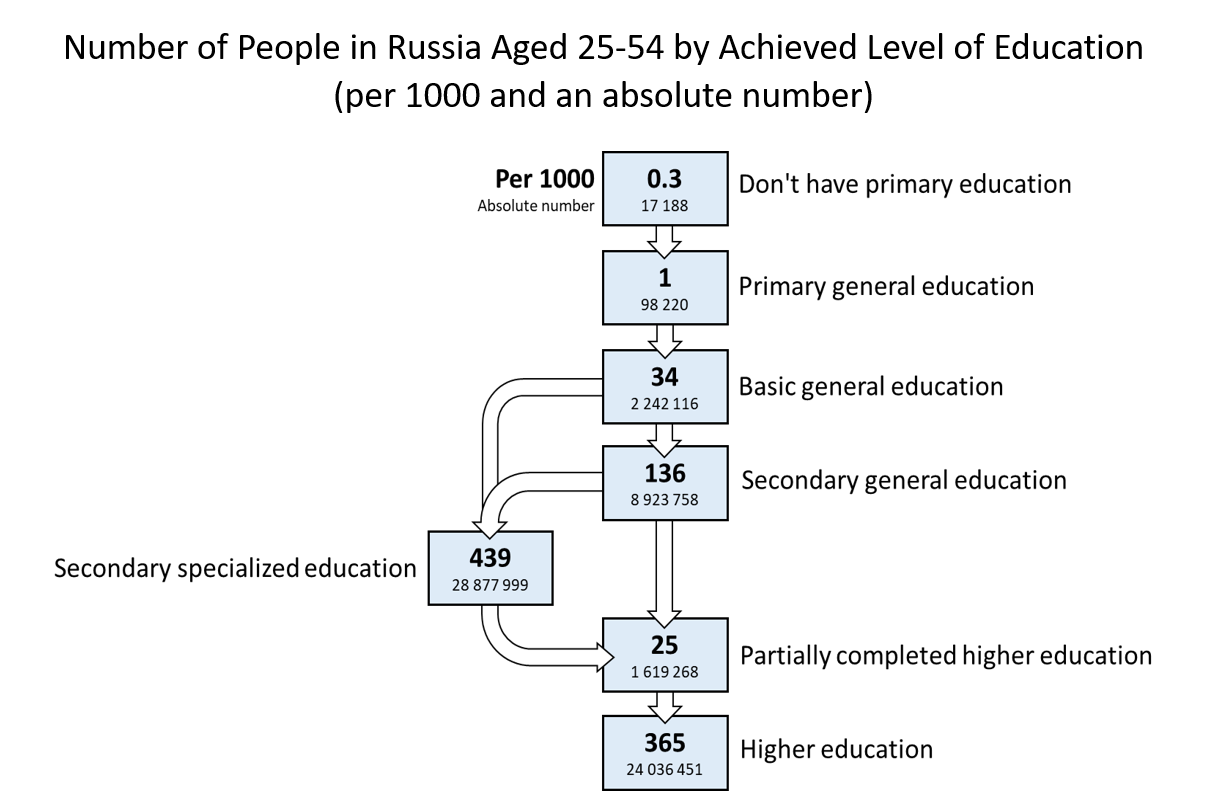
\includegraphics[width=5in]{graph_1c.png}
			% plot 1
		\end{minipage}
			\caption{Labor Force Distribution by Educational Level (Rosstat)}\label{fig:1.1c}
	\end{figure}
\end{center}


\vspace{-2em}


Figure \ref{fig:1.1b}  shows the percentage of 17-25-year-olds in the Russian federation enrolled in university programs. The figure shows that even as university enrollment had expanded very rapidly since 2000, when 23\% of the age group were enrolled, university enrollment appears to have peaked and then declined. Women reached a peak of 41.1\% enrollment in 2010 and had declined to 34.8\% by 2016. Men reached a peak of 30.4\% enrollment in 2013 and have declined more slowly to 28.9\% in 2016. Every 0.1\% of change is roughly equivalent to 120,000 individuals. Figure \ref{fig:1.1c} indicates the educational attainment of the population segment 25 to 54 years (who would mostly have finished their formal education and within the retirement age - 55 for women until the recently introduced reforms). Figure \ref{fig:1.1c}  shows less than 14\% of the labor force with final attainment of secondary general education (academic High School) - the main choice is between vocational education (nearly 45\%) and university education (about 40\%). Finally, Figure \ref{fig:1.1d}  shows that on cognitive attainment at Grade 9, Russian students are already at par with OECD students (PISA scores are designed with an OECD mean of 500); what comes in later education levels and the labor market is the crucial issue for convergence with OECD on human capital wealth levels. 

A detailed analysis of the returns to education in the Russian Federation will provide insights into the stylized facts mentioned above. Together with other research being implemented by the World Bank and by researchers outside of the World Bank, the purpose of this analysis is to come up with a set of evidence based policy recommendations to enhance the human capital wealth of the Russian Federation. 

 
\section{Data}

For country level analysis, we use the Russian Longitudinal Monitoring Survey (RLMS) - the only representative Russian survey with a sizable panel component allowing for a dynamic analysis \parencite{kozyreva_081._2015}. The data are notable for their reliability, diversity, and applicability to a variety of research questions. The RLMS embraces information on people's income and expenditure structure, their material well-being, educational and occupational behavior, health state and nutrition, migration, etc.  RLMS sampling procedures have been thoroughly and extensively described elsewhere \parencite{kozyreva_081._2015}. The present research uses all 23 waves (1994 - 2018) that are available as of \today. The sub-sample selected for empirical investigation in this paper consists of working individuals aged 25-64 who are out of school and have positive labor market experience and income. 
\\

\section{Estimation}

Our empirical analysis present results for the general working population of the Russian Federation aged 25-64 and by gender. We use a basic Mincerian specification shown in equation \eqref{eq:1.1}: 


\begin{flalign}\label{eq:1.1} 
Log(Wage) = b_0 + b_1\cdot Educ + b_2\cdot Exp + b_3\cdot Exp^2 + b_4\cdot Gender + \epsilon
\end{flalign}



\noindent
where $Log(Wage)$ is a logarithm of monthly wage, $Educ$ stands for the years of education or highest attained level of education, $Exp$ and $Exp^2$ reflect the years of working experience and its quadratic term respectively, $Gender$ is a dummy variable for gender, $b_0$ is an intercept, $b_1 ... b_n$ are the respective slope estimates, $\epsilon$ refers to a normally distributed error term.

%\subsection{Measures}

\textbf{Dependent variable}

For the dependent variable, we used the logarithm of an average monthly wage within the past year on a person's primary job (J13.2 variable in the RLMS dataset). If a person had an additional job, the maximum wage value among the two (J13.2 and J40) was selected for the analysis. In the waves from 1994 to 1996, the question mentioned above was absent; for those waves, we exploited a variable about the average amount of money earned by a respondent within the past 30 days (J10) as a reasonable approximation.

\textbf{Independent variables}

The present research uses both metric (measured in years) and categorical education variables. The metric version was created by assigning the average expected number of years corresponding to each attained education level. For the categorical version (EDUC), we distinguished three categories: \textit{(1) secondary, (2) vocational, and (3) higher}. Incomplete levels were incorporated into the respective upper categories (e.g., incomplete higher - into higher). We are interested in exploring returns to education in general, and vocational and higher education. Estimations of premiums to primary and secondary schooling levels are technically unreachable to us since the number of adults without primary education, and the number of adults with only primary level is minuscule in the general population. 

The experience variable was calculated as a difference between current age and years of education minus $6$. Gender was included in the specification in the form of a dichotomous dummy variable with "$1$" standing for females, "$0$" - for males.

% \subsection{Findings from Estimation of Mincerian Equation}

Figure \ref{fig:1.2} shows rates of overall and gender-wise returns to education in Russia in 1994-2018: percentage increment in a person's earnings due to one additional year of schooling (exact estimation results available on github site for this paper). Overall, one can notice a moderate curved growth in returns to education in Russia, achieving its peak in the early 2000s, which is followed by a downward pattern. Education payoffs for women are higher than those of men, but the difference appears to have narrowed in recent years (see tables with 95\% confidence intervals of regression coefficients on gihub site for this paper).

\begin{figure}[H]
 \centering
 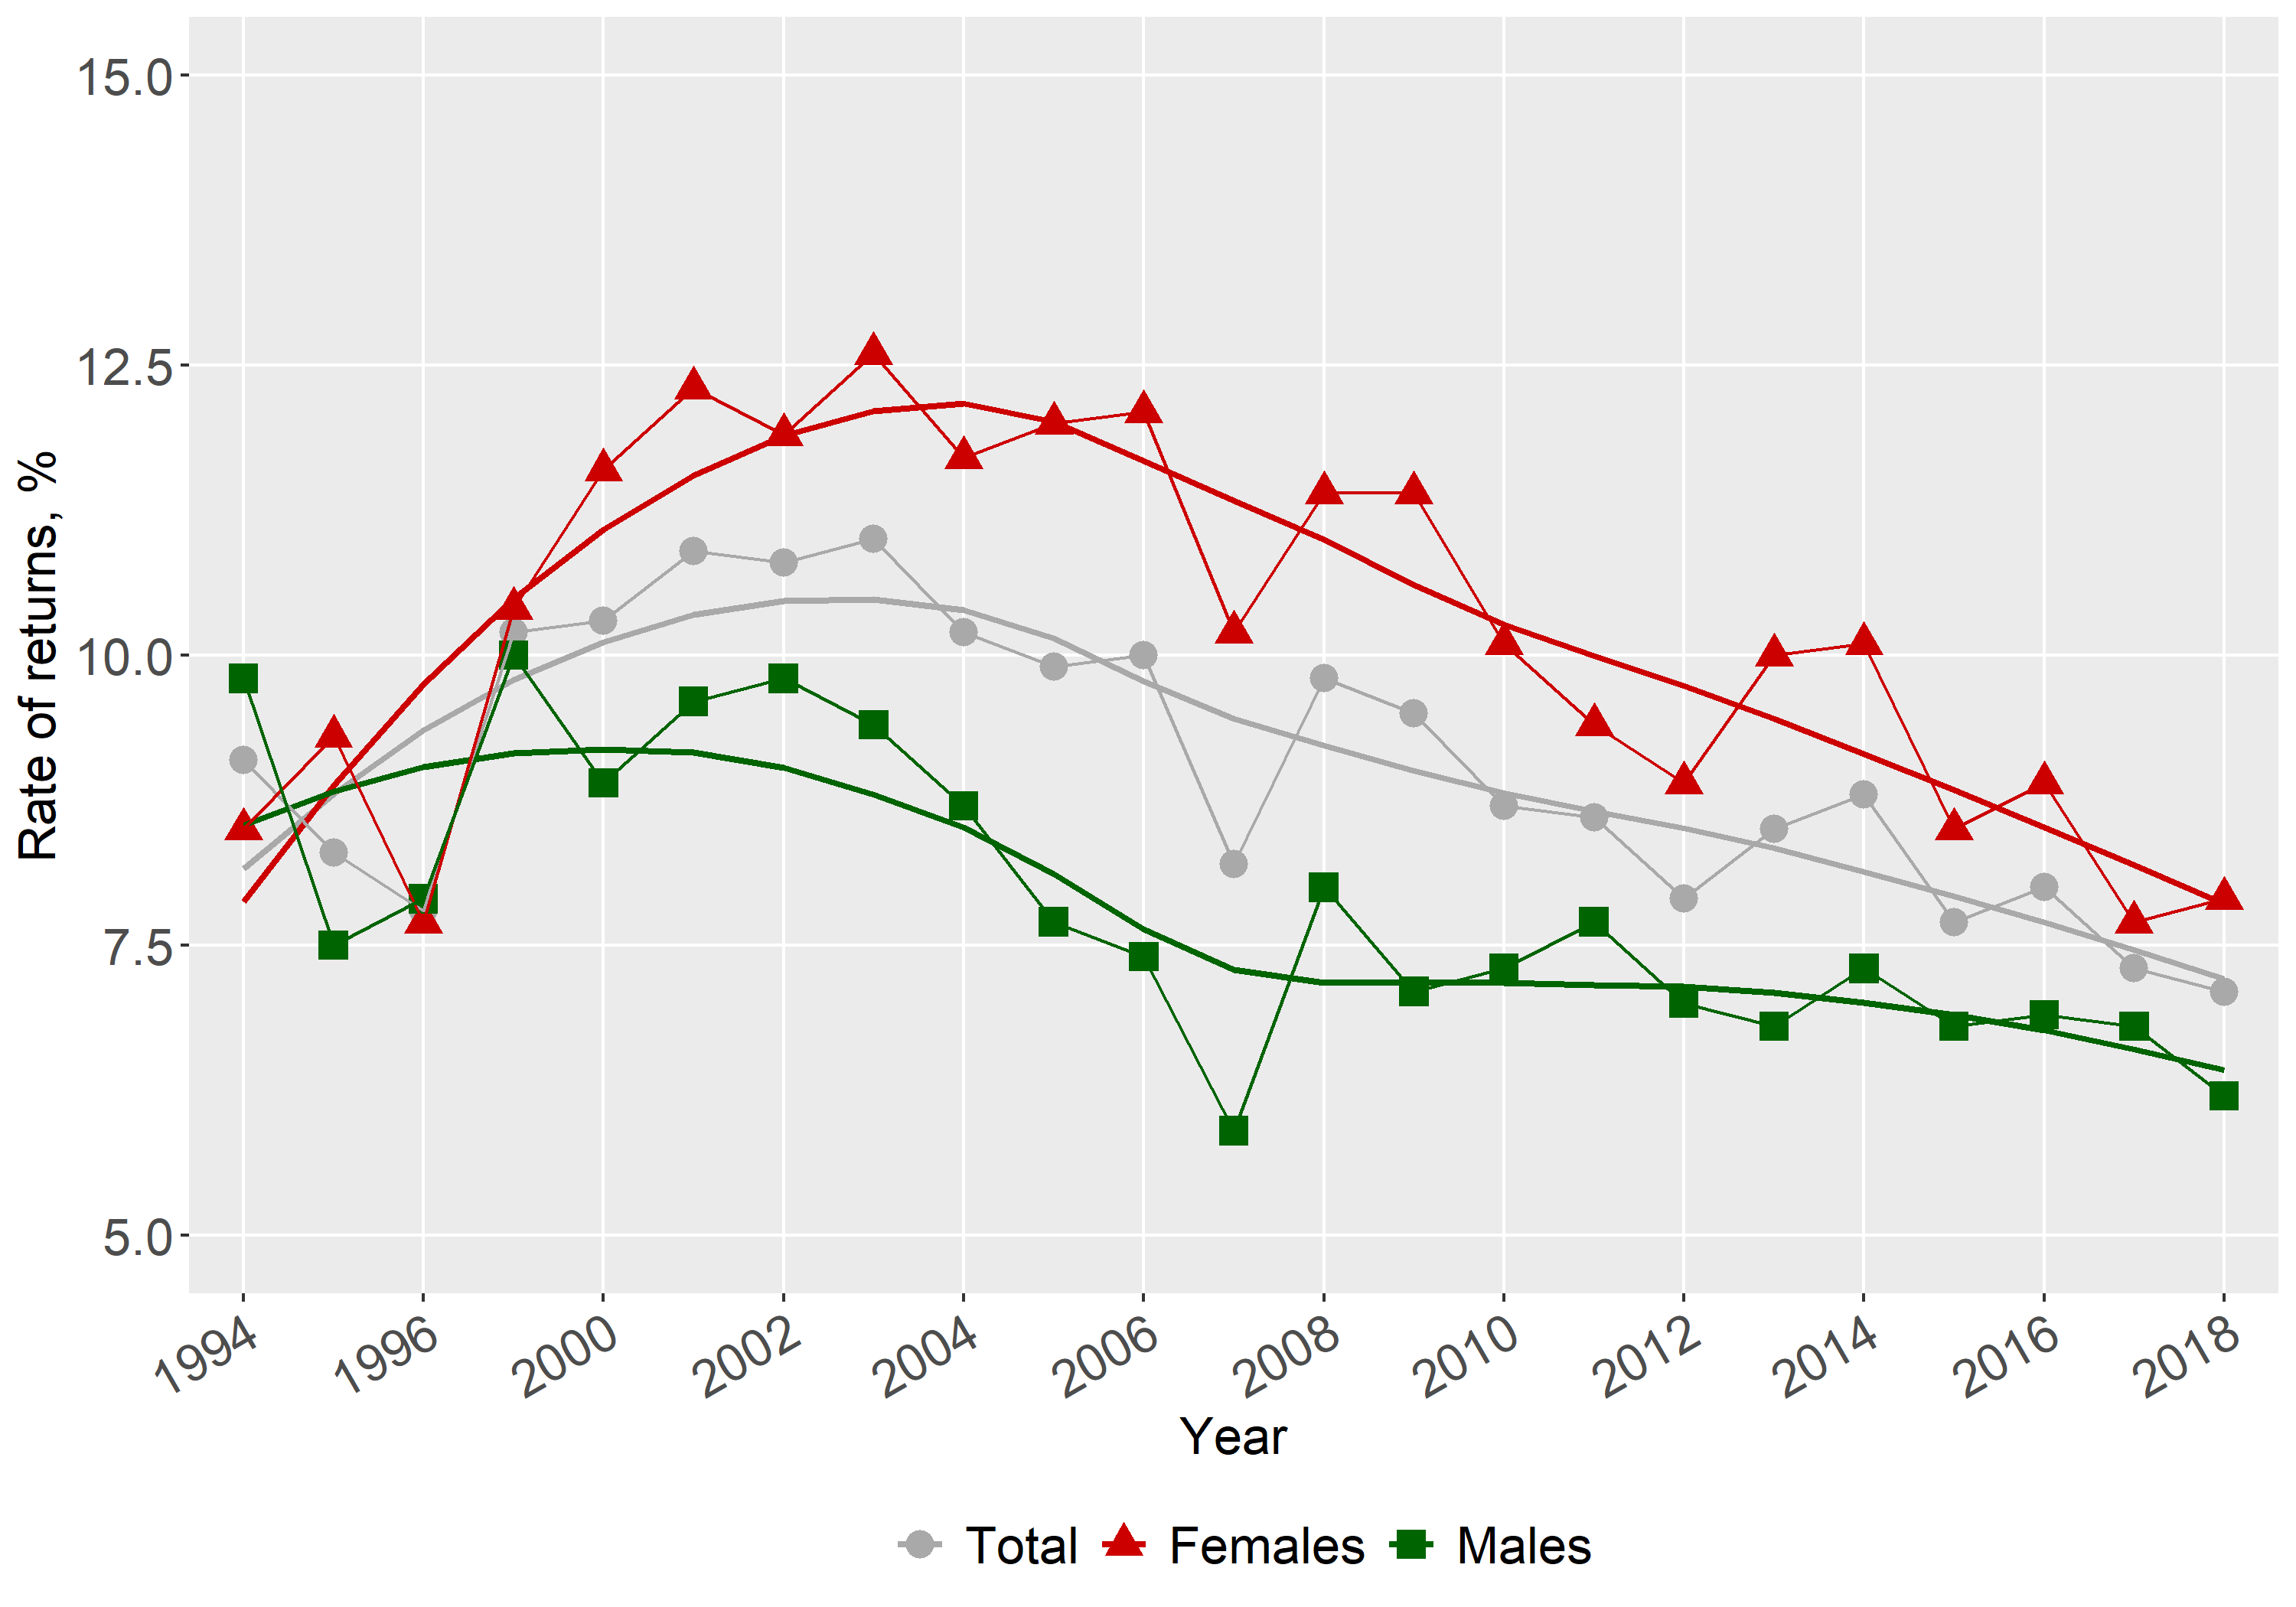
\includegraphics[width=\textwidth, height=300pt]{re_edu.png}
 \caption{Rates of Returns to Education in Russia, RLMS 1994-2018}\label{fig:1.2}
\end{figure}

We are particularly interested in the returns to specific levels of education, estimated through a series of dummy variables. Using Secondary Education completed as the base or omitted dummy for purpose of interpretation, we use dummies for Vocational Education and for Higher Education. The specification is presented in equation \eqref{eq:1.2}: 

\begin{flalign}\label{eq:1.2} 
Log(Wage) = a_0 + a_1\cdot D_{Voc} + a_2\cdot D_{Higher} + a_3\cdot Exp + a_4\cdot Exp^2 + a_5\cdot Gender + \epsilon
\end{flalign}


Figure \ref{fig:1.3}, panel (a) displays rates of returns to Higher and Vocational education (as compared to Secondary education) in Russia for the period 1994-2018. The results suggest that on average wage premiums to university education in Russia are roughly 3-5 times greater than to vocational schooling. The observed trend for premiums to both Vocational and Higher education levels is similar to the trend for education in general with the following peaks: 83\% for Higher education and 26\% for Vocational education compared to the average earnings of workers with a Secondary education. The interesting pattern to note from panel \ref{fig:1.3a} is the apparent co-movement of vocational education and higher education - the higher education smoothing curve turns a bit more sharply than the one for vocational education, but their movement is matching, even at second-order levels of smoothness. Further, even though higher education premium remains much above the premium for vocational education, there is a perceptible narrowing of the difference in recent years. Panel \ref{fig:1.3b}, which is drawn from a presentation made by Marina Telezhkina at the WB-HSE Summer School on the Economics of Education in July 2019, shows the interesting pattern of higher education enrollment rates for the population of 17-25 year old. Panel \ref{fig:1.3b} shows the downturn in returns reflected in enrollments, with the peak in enrollments coming about 10 years later. 

\begin{figure}[H]
\caption{\textbf{Rates of Returns to Higher and Vocational Education in Russia, RLMS 1994-2018}}\label{fig:1.3}
         \centering
         \begin{subfigure}[b]{0.5\textwidth}
                 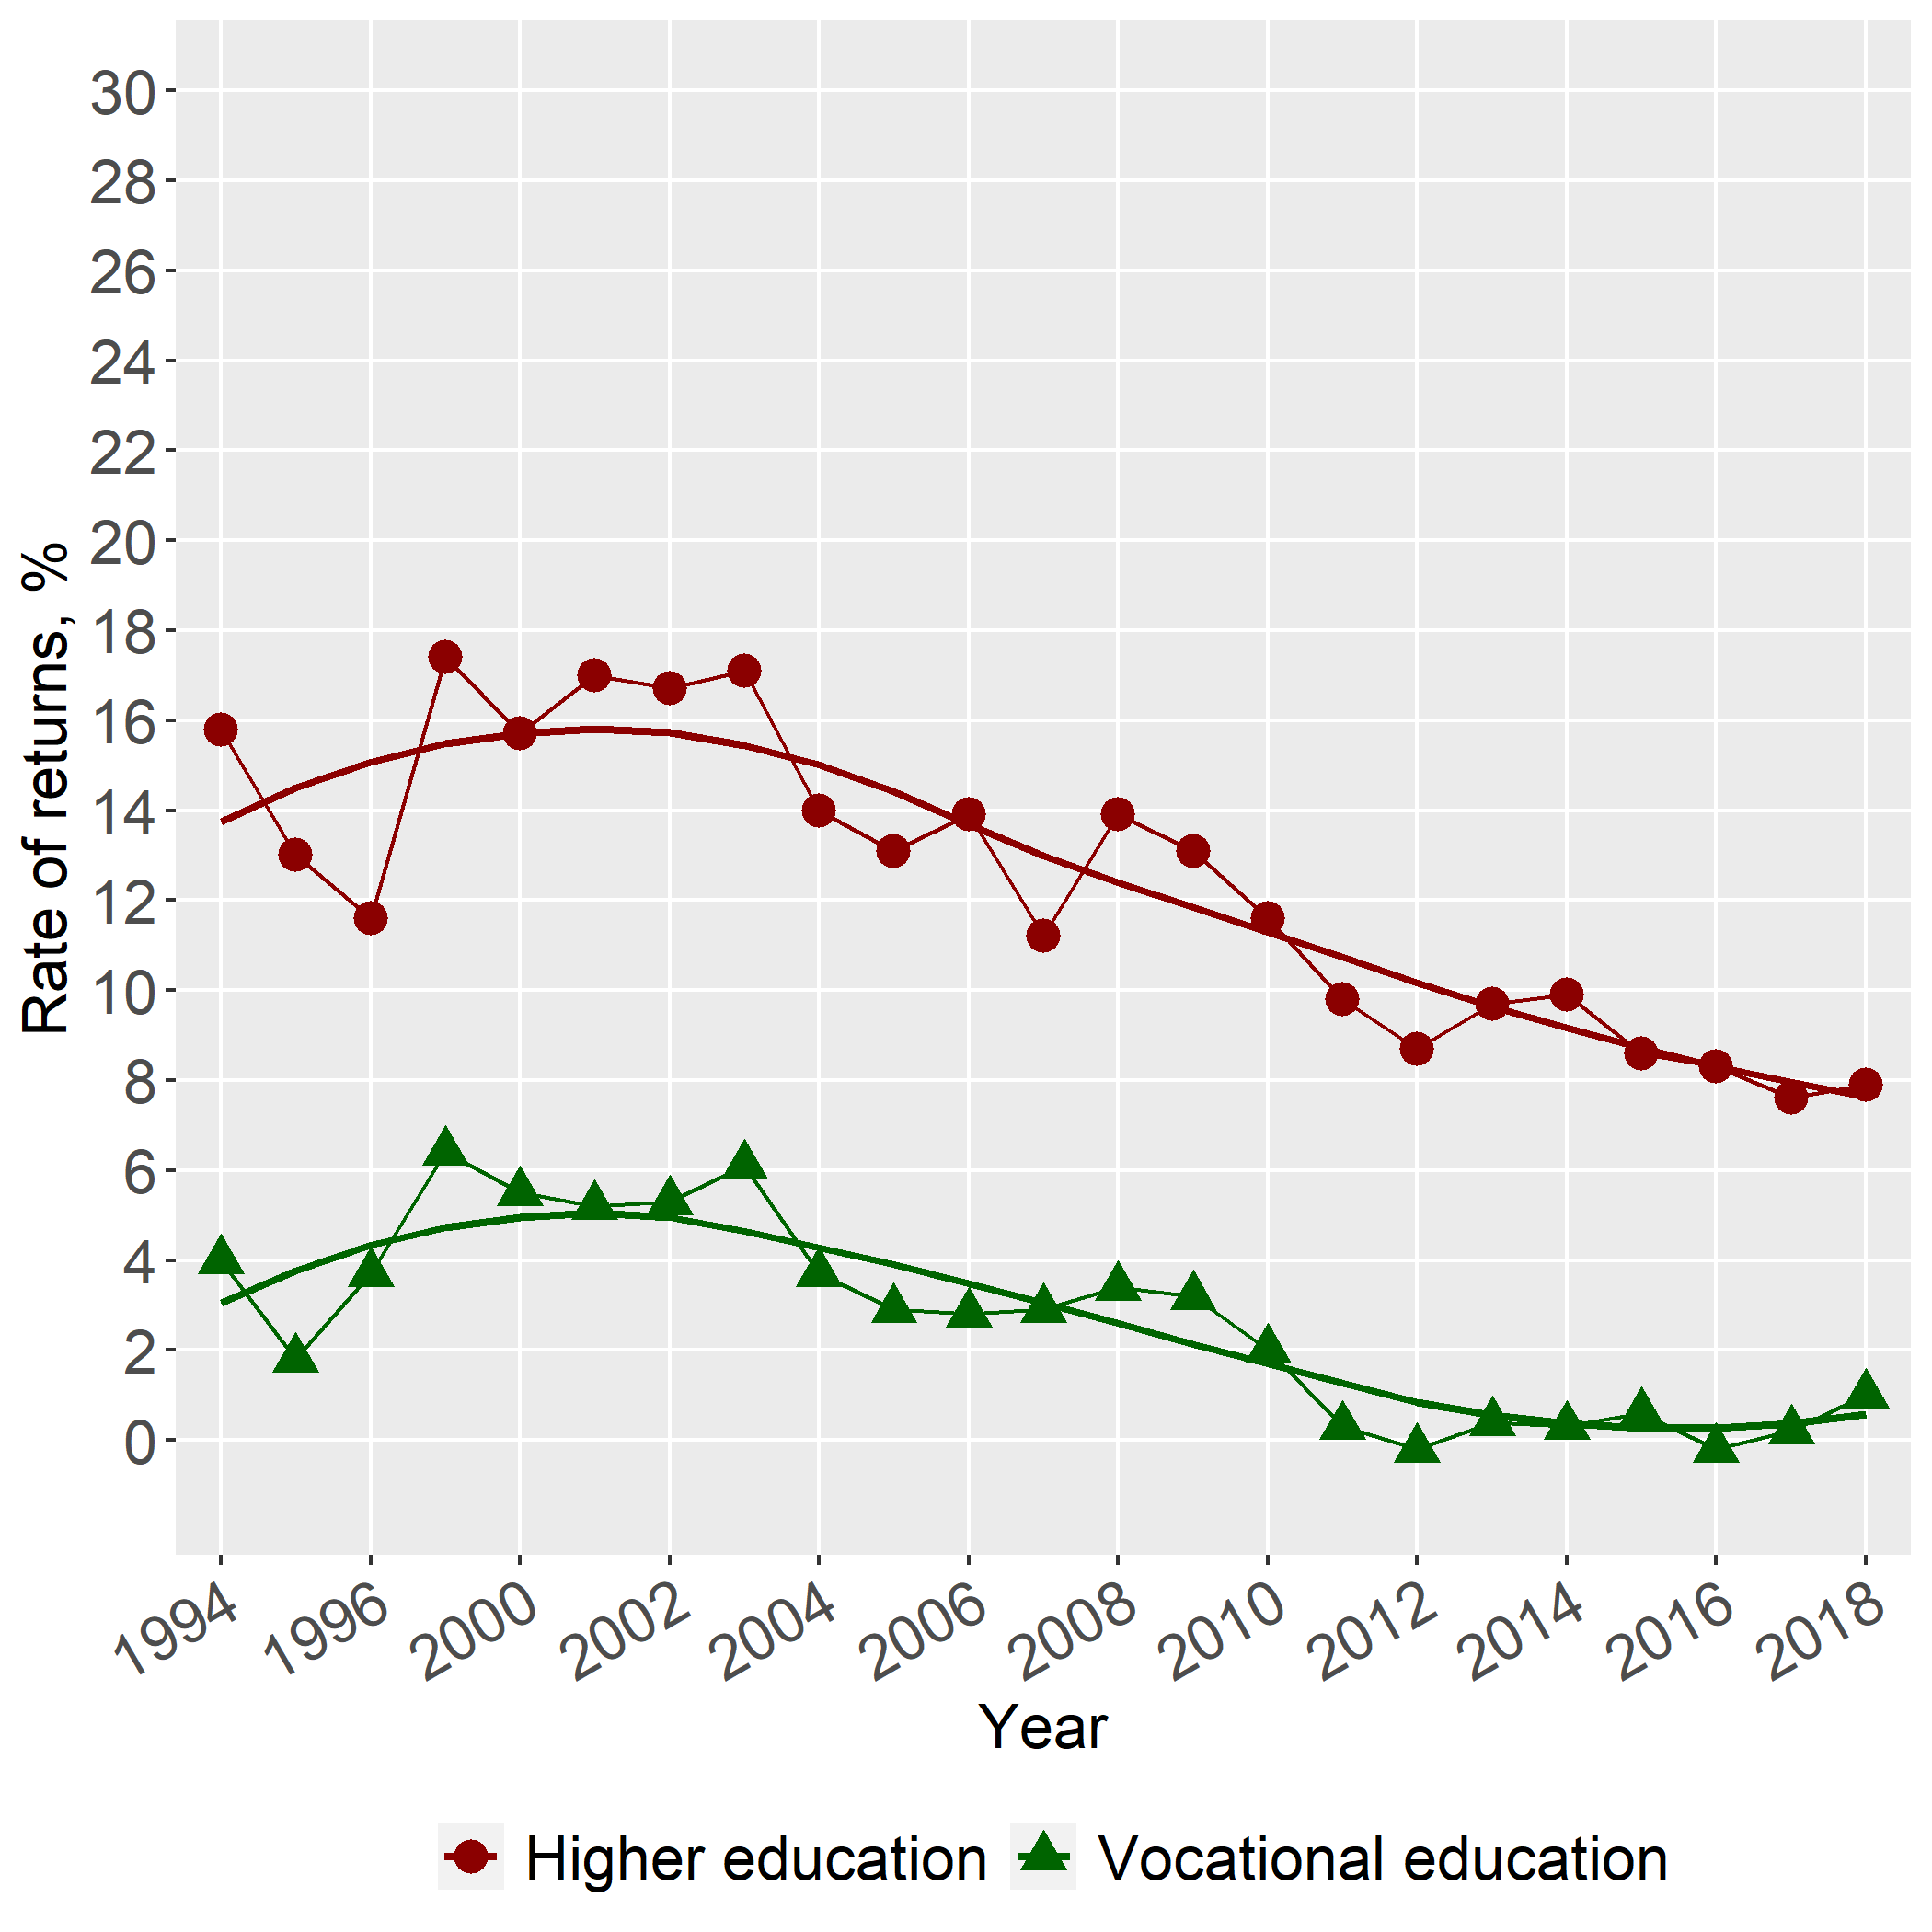
\includegraphics[width=\textwidth]{re_HE_all.png}
                 \caption{Rates of Return}
                 \label{fig:1.3a}
         \end{subfigure}%
         ~ %add desired spacing between images, e. g. ~, \quad, \qquad, \hfill etc.
           %(or a blank line to force the subfigure onto a new line)
         \begin{subfigure}[b]{0.5\textwidth}
                 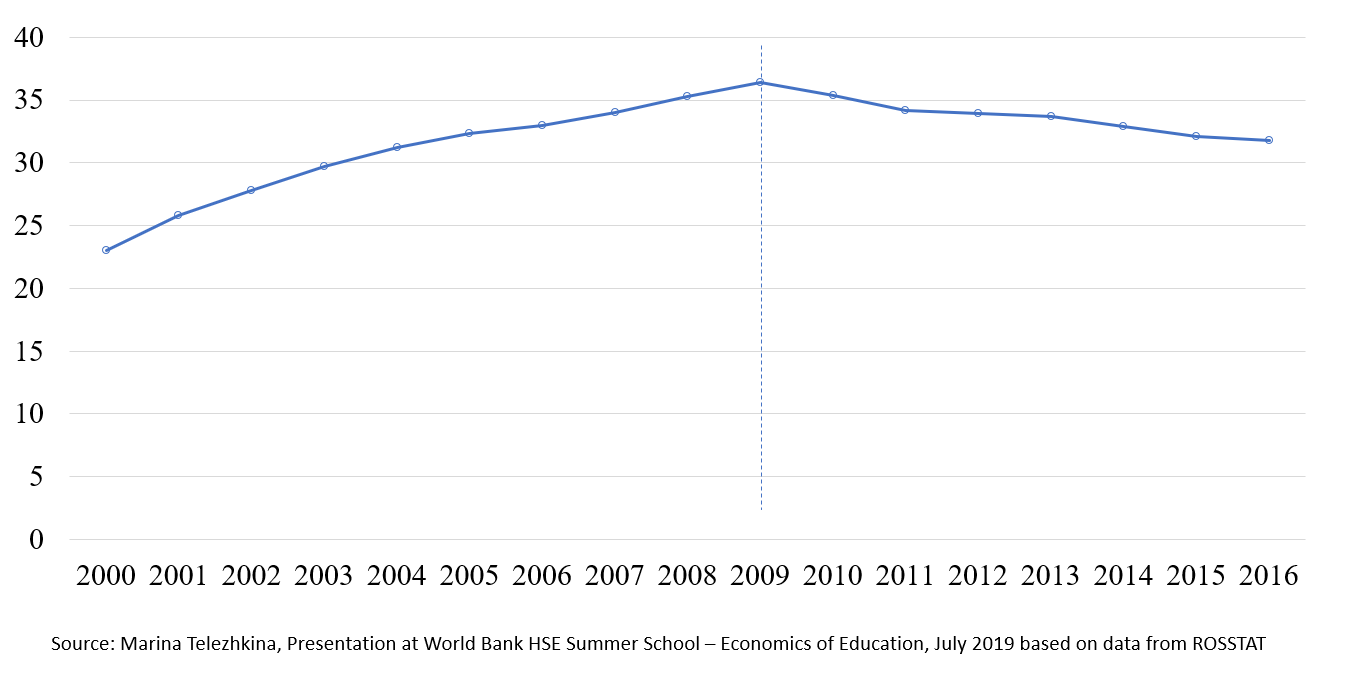
\includegraphics[width=\textwidth]{telezhkina.png}
                 \caption{Enrollment in Higher Education}
                 \label{fig:1.3b}
         \end{subfigure}
     \end{figure}

When estimated separately by gender, we find trend variation by gender. The results from estimation of earnings functions show that payoffs to Higher education for males varied from 45\% to 76\%, whereas women's returns are described by an inversely U-shaped pattern, reaching their maximum of 104\% in 2001. Within roughly the last 5 years, wage premiums to higher education for women have stabilized around the level of men (~50\%).  Gender wise enrollment rates in higher education (not shown) ten years later appears to match the differences in rates of return, strengthening the hypothesis that market rates of return to education in Russia do indeed influence individual continuing school decisions. 

A similar comparative picture is observed with respect to vocational education, albeit with a different kind of variation by gender (see Figure \ref{fig:1.4}): returns for males are almost flat within the time period while returns for females shows a concave pattern. The overall outcome concerning payoffs to schooling isolated by gender has been confirmed in a similar fashion by past studies \parencite[e.g.,][]{cheidvasser_006._2007}.

\begin{figure}[H]
  \begin{minipage}[b]{.5\linewidth}
     \centering
     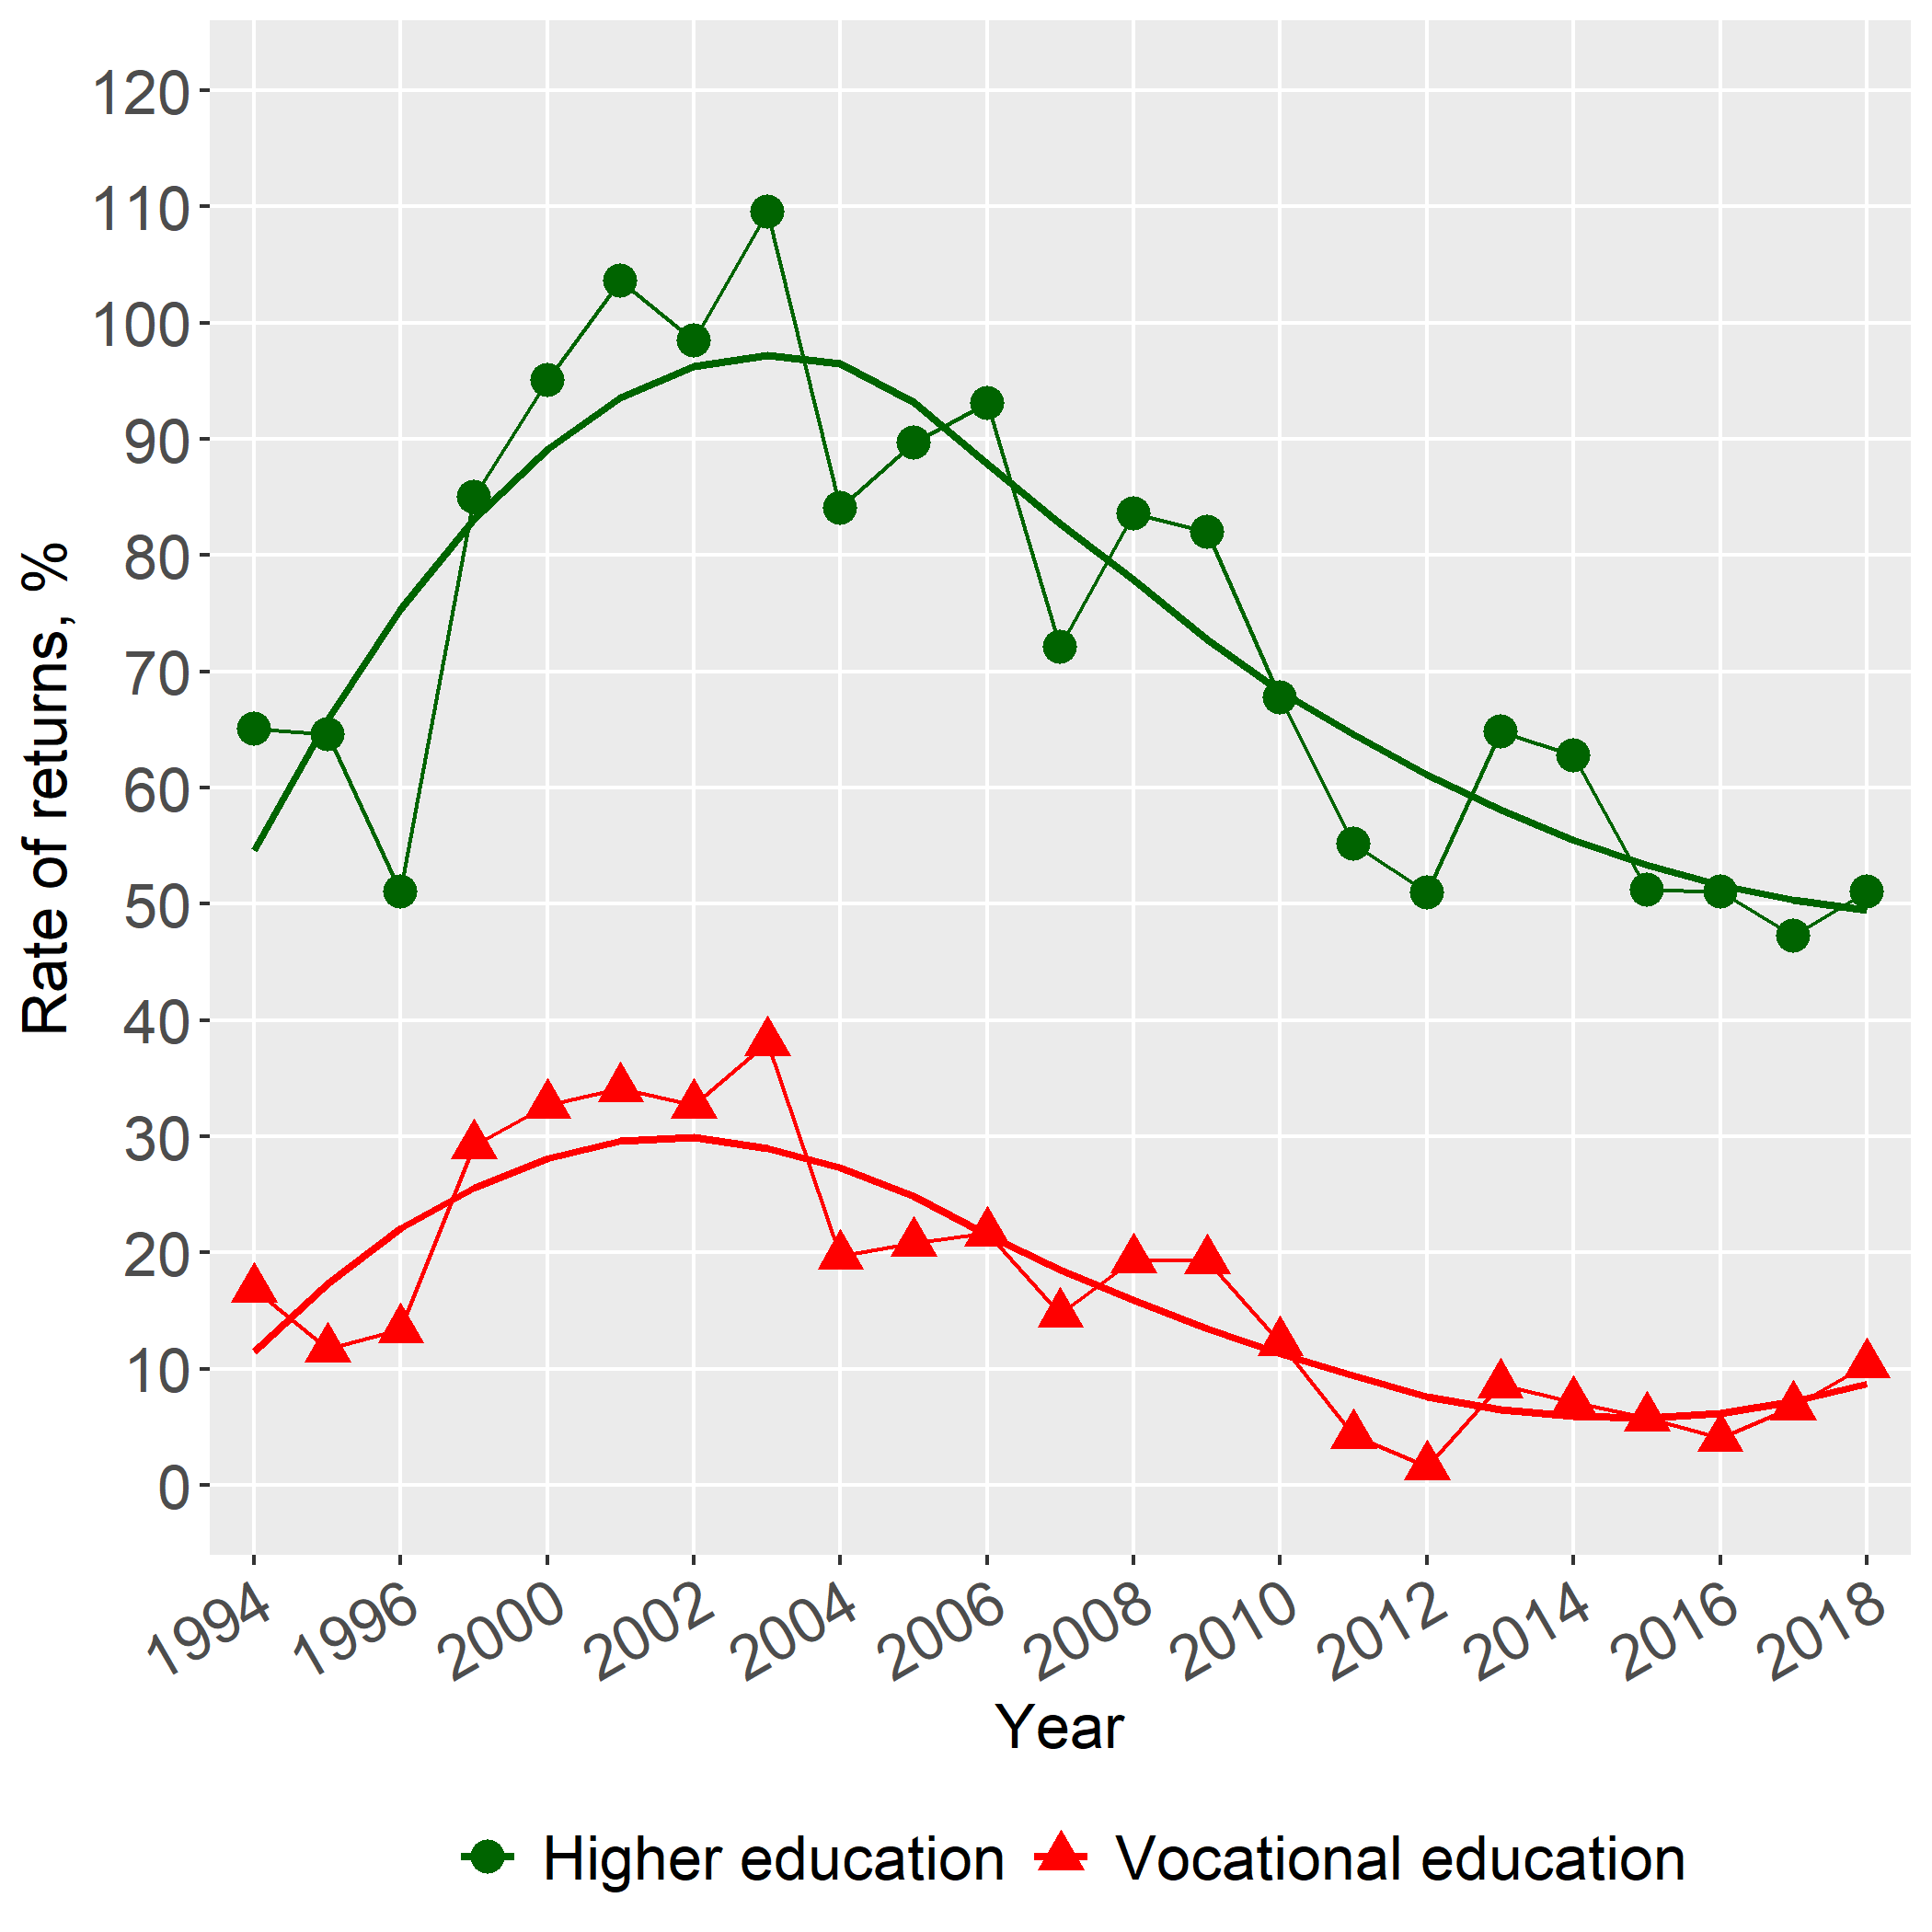
\includegraphics[width=\textwidth]{re_HE_f.png}
     % plot 1
     \subcaption{Females}\label{fig:1.4a}
  \end{minipage}
  \hfill
  \begin{minipage}[b]{.5\linewidth}
     \centering
     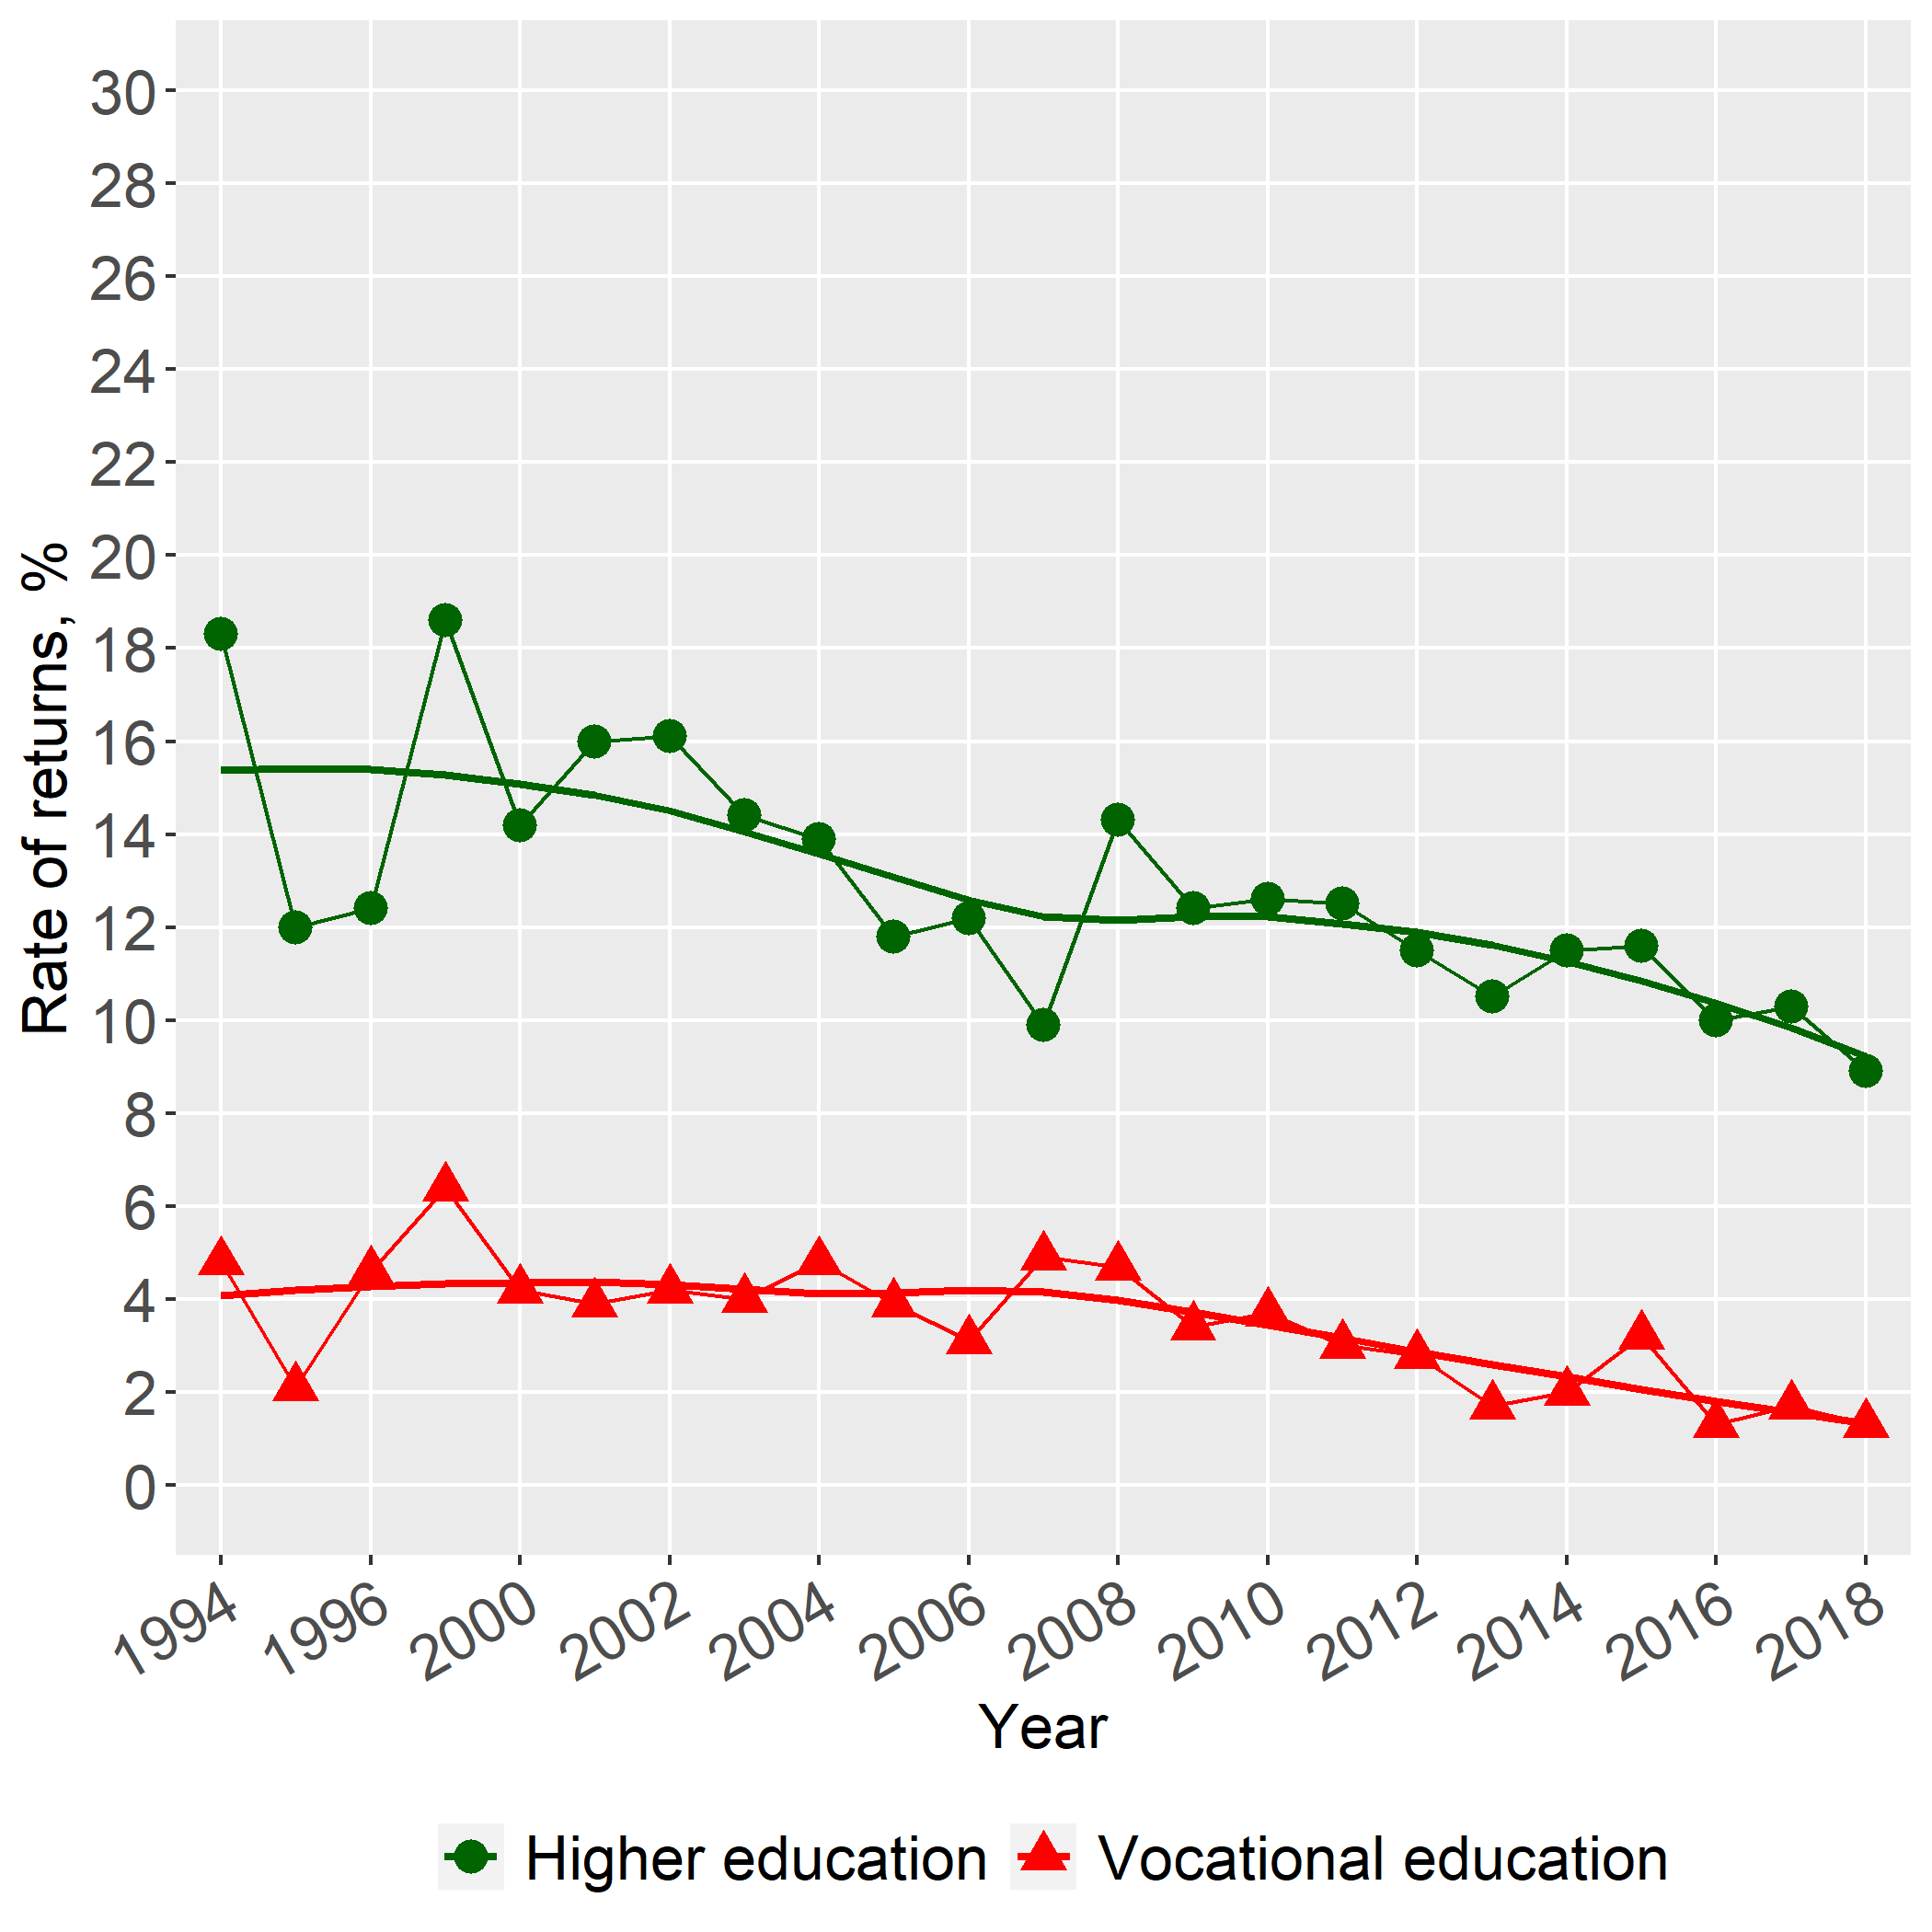
\includegraphics[width=\textwidth]{re_HE_m.png}
     % plot 2
     \subcaption{Males}\label{fig:1.4b}
  \end{minipage}
  \caption{Rates of Returns to Higher and Vocational Education in Russia, RLMS 1994-2018}\label{fig:1.4}
\end{figure}

\newpage 

\printbibliography

\end{document}
